\documentclass[conference]{IEEEtran}
\IEEEoverridecommandlockouts

\usepackage{cite}
\usepackage{amsmath,amssymb,amsfonts}
\usepackage{algorithmic}
\usepackage{graphicx}
\usepackage{textcomp}
\usepackage{xcolor}
\def\BibTeX{{\rm B\kern-.05em{\sc i\kern-.025em b}\kern-.08em
    T\kern-.1667em\lower.7ex\hbox{E}\kern-.125emX}}
\begin{document}

\title{Single-Point GPS Positioning}

\author{\IEEEauthorblockN{Mazen Elaraby}
\IEEEauthorblockA{\textit{Department of Electrical and Computer Engineering} \\
\textit{Queen's University}\\
Kingston, Canada 
}}

\maketitle

\begin{abstract}
Global Navigation Satellite System (GNSS) based positioning is a cornerstone of modern navigation, providing absolute localization critical for applications such as land surveying, autonomous vehicles, and aerial robotics. Unlike relative localization methods, GNSS offers globally referenced positioning that mitigates the drift accumulation inherent to dead reckoning, LiDAR, and visual odometry. Single-Point GPS Positioning (SPP) is a fundamental GNSS-based method that estimates receiver position, velocity, clock bias, and clock drift. While SPP remains indispensable, its accuracy is inherently limited by factors such as multipath effects, jamming, and spoofing.

This paper investigates state estimation techniques for SPP, focusing on nonlinear least squares (NLS) and Kalman filtering. NLS, a deterministic parameter estimation method, optimally solves each epoch independently, while Kalman filtering provides a recursive framework for sequential estimation under dynamic conditions. We further explore the impact of numerical conditioning on state estimation and evaluate multiple matrix inversion techniques, including Normal Equations, QR Decomposition, and Singular Value Decomposition (SVD). Additionally, we introduce Dilution of Precision (DOP)-Gated Epoch Rejection, a heuristic method designed to enhance robustness by mitigating the effects of poorly conditioned epochs. Empirical evaluations demonstrate the effectiveness of these approaches in improving SPP accuracy and stability.
\end{abstract}

\begin{IEEEkeywords}
GNSS positioning, Single-Point Positioning (SPP), state estimation, nonlinear least squares, Kalman filtering, numerical conditioning, matrix inversion, GPS navigation, Dilution of Precision (DOP), real-time localization.
\end{IEEEkeywords}

\section{Introduction}

Global Navigation Satellite System (GNSS) based positioning has become an indispensable component of modern navigation solutions. From land surveying and autonomous ground vehicles to aerial robotics and maritime navigation, GNSS provides critical positioning data that serves as the foundation for numerous applications. Unlike relative localization methods such as dead reckoning, LiDAR odometry, or visual-inertial navigation, GNSS offers an absolute position fix referenced to a globally consistent coordinate system. This absolute nature makes GNSS-based positioning particularly advantageous in scenarios where drift accumulation in relative navigation methods would otherwise degrade accuracy over time.

Single-Point GPS Positioning (SPP) is a fundamental GNSS-based localization method that estimates the receiver’s position and velocity while also accounting for clock bias and clock drift. Despite the simplicity of its implementation, SPP plays a vital role in providing robust location estimates across a wide range of applications. However, like any GNSS-based system, SPP is subject to inherent limitations, including multipath effects, signal jamming, and spoofing attacks, all of which can introduce positioning errors or even cause complete GNSS outages. While alternative localization techniques such as inertial navigation systems (INS), LiDAR-based simultaneous localization and mapping (SLAM), or radar odometry can help bridge GNSS outages, none of these methods can completely replace the global and absolute positioning capability of GNSS.

Relative navigation methods, such as dead reckoning or LiDAR-based odometry, suffer from significant drawbacks that limit their standalone applicability. Dead reckoning, which relies on accelerometers and gyroscopes, accumulates drift errors over time, making it unsuitable for long-term navigation without external corrections. Visual and LiDAR-based odometry, while effective in structured environments, can fail in textureless, feature-poor, or dynamic conditions, such as in open water, fog, or environments with rapid scene changes. Moreover, radar-based odometry, while robust in adverse weather conditions, is limited by its angular resolution. In contrast, GNSS-based positioning remains viable across diverse environments, providing global coverage with predictable error characteristics. Additionally, GNSS accuracy can be significantly enhanced through augmentation techniques such as Real-Time Kinematic (RTK) positioning, Differential GNSS (DGNSS), and Precise Point Positioning (PPP), which reduce the nominal 10-meter accuracy of Single-Point Positioning to centimeter-level precision under ideal conditions.

At its core, Single-Point GPS Positioning is a state estimation problem that can be effectively solved using nonlinear least squares (NLS) and Kalman filtering. NLS, a deterministic parameter estimation method, solves each epoch independently by minimizing the residuals between measured and predicted pseudoranges. Kalman filtering, in contrast, is a recursive estimator, continuously updating state estimates in real time while accounting for measurement noise and system dynamics. The widespread adoption of these methods stems from their mathematical rigor, numerical stability, and extensive hardware optimization, ensuring feasibility for real-time GNSS positioning applications.

This paper contributes to the advancement of Single-Point GPS Positioning by exploring multiple state estimation approaches, including nonlinear least squares solved via a Gauss-Newton-based solver. Given the numerical conditioning challenges inherent to GNSS state estimation, we investigate multiple matrix inversion techniques, including Normal Equations, QR Decomposition, and Singular Value Decomposition (SVD), along with their weighted variants. Additionally, Kalman filtering is employed as an alternative estimation method. To further address system conditioning issues, a heuristic method called Dilution of Precision (DOP)-Gated Epoch Rejection is introduced, which selectively discards poorly conditioned epochs to improve estimation robustness. The remainder of this paper presents a detailed analysis of these methods, along with empirical evaluations of their performance in real-world GNSS scenarios.

\section{Implementation Details}

\subsection{Problem Setup}

Our problem is to jointly estimate the receiver's position \( \mathbf{x} = [x, y, z]^T \), velocity \( \mathbf{v} = [v_x, v_y, v_z]^T \), clock bias \( b_r \), and clock drift \( d_r \) using pseudorange and Doppler measurements from at least four visible satellites.

\textbf{Provided Data:}
\begin{itemize}
    \item \textbf{Satellite Positions and Velocities:} \\
    For each visible satellite \( m \), the position \( \mathbf{x}^m = [x^m, y^m, z^m]^T \) and velocity \( \mathbf{v}^m = [v_x^m, v_y^m, v_z^m]^T \) in the Earth-Centered, Earth-Fixed (ECEF) frame are provided.
    
    \item \textbf{Pseudorange Measurements:} \\
    The pseudorange \( \rho_c^m \) to each satellite \( m \) is measured.
    
    \item \textbf{Doppler Measurements:} \\
    The Doppler shift \( D^m \) is measured, which is related to the pseudorange rate \( \dot{\rho}^m \).
\end{itemize}

\textbf{Pseudorange Equation:}
\begin{equation}
\rho_c^m = \|\mathbf{x} - \mathbf{x}^m\| + b_r + \varepsilon_\rho^m
\end{equation}
\begin{itemize}
    \item \( \rho_c^m \): Measured pseudorange to the \( m \)-th satellite.
    \item \( \|\mathbf{x} - \mathbf{x}^m\| \): True geometric range between the receiver and the \( m \)-th satellite.
    \item \( b_r = c\delta t_r \): Error in range due to the receiver's clock bias, where \( c \) is the speed of light and \( \delta t_r \) is the receiver clock bias in seconds.
    \item \( \varepsilon_\rho^m \): Error in the pseudorange measurement (e.g., atmospheric delays, multipath).
\end{itemize}

\textbf{Doppler Effect Equation:}
\begin{equation}
D^m = \frac{\{(\mathbf{v}^m - \mathbf{v}) \cdot \mathbf{1}^m\} L}{c}
\end{equation}
\begin{itemize}
    \item \( D^m \): Doppler shift observed by the receiver for the \( m \)-th satellite.
    \item \( \mathbf{v}^m \): Velocity of the \( m \)-th satellite in the ECEF frame.
    \item \( \mathbf{v} \): True velocity of the receiver in the ECEF frame.
    \item \( \mathbf{1}^m \): Unit vector in the line of sight from the receiver to the \( m \)-th satellite.
    \item \( L \): Transmitted frequency of the satellite signal.
    \item \( c \): Speed of light.
\end{itemize}

\textbf{Pseudorange Rate Equation:}
\begin{equation}
\dot{\rho}^m = -\frac{D^m c}{L}
\end{equation}
\begin{itemize}
    \item \( \dot{\rho}^m \): Pseudorange rate (rate of change of pseudorange) for the \( m \)-th satellite.
    \item \( D^m \): Doppler shift for the \( m \)-th satellite.
    \item \( c \): Speed of light.
    \item \( L \): Transmitted frequency of the satellite signal.
\end{itemize}

\textbf{Pseudorange Rate Equation:}
\begin{equation}
\begin{split}
\dot{\rho}^m &= 1_x^m (v_x - v_x^m) + 1_y^m (v_y - v_y^m) \\
&\quad + 1_z^m (v_z - v_z^m) + c\delta t_r + \varepsilon_\rho^m
\end{split}
\end{equation}
\begin{itemize}
    \item \( \dot{\rho}^m \): Pseudorange rate for the \( m \)-th satellite.
    \item \( 1_x^m, 1_y^m, 1_z^m \): Components of the unit vector \( \mathbf{1}^m \) in the line of sight from the receiver to the \( m \)-th satellite.
    \item \( v_x, v_y, v_z \): Components of the receiver's velocity.
    \item \( v_x^m, v_y^m, v_z^m \): Components of the \( m \)-th satellite's velocity.
    \item \( c\delta t_r \): Receiver clock drift in meters per second, where \( \delta t_r \) is the receiver clock drift in seconds.
    \item \( \varepsilon_\rho^m \): Error in the pseudorange rate measurement.
\end{itemize}

\begin{figure}[htbp]
\centerline{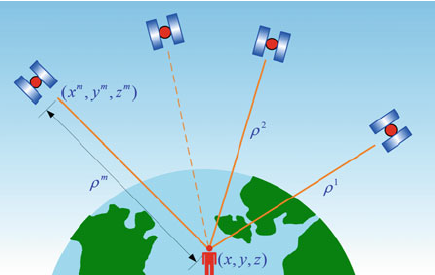
\includegraphics[width=0.4\textwidth]{fig.png}}
\caption{Problem Setup.}
\label{fig:setup}
\end{figure}

\subsection{Linearization of System of Nonlinear Equations for Estimation}

To estimate the receiver's position, velocity, clock bias, and clock drift, we start with a system of nonlinear equations derived from pseudorange and Doppler measurements. These equations are linearized using a Taylor series expansion to simplify the estimation process.

\subsubsection*{Linearization of Pseudorange Equation}

The pseudorange equation is nonlinear due to the geometric range term. To linearize it, we use a Taylor series expansion around the current best estimate of the receiver's position, \( \mathbf{x}_{EST} = [x_{EST}, y_{EST}, z_{EST}]^T \). For any function \( f(x, y, z) \), the Taylor series expansion around \( (x_i, y_i, z_i) \) is given by:

\begin{equation}
\begin{split}
f(x, y, z) &= f(x_i, y_i, z_i) + \frac{\partial f}{\partial x}\bigg|_{x_i, y_i, z_i}(x - x_i) \\
&\quad + \frac{\partial f}{\partial y}\bigg|_{x_i, y_i, z_i}(y - y_i) + \frac{\partial f}{\partial z}\bigg|_{x_i, y_i, z_i}(z - z_i) + \text{H.O.T}
\end{split}
\end{equation}

Applying this to the pseudorange equation, we linearize it around \( \mathbf{x}_{EST} \) and get the compact form for the the difference between the measured and estimated pseudorange is:

\begin{equation}
\delta \rho_c^m = \left( \mathbf{1}_{EST}^m \right)^T \delta \mathbf{x} + \delta b_r + \tilde{\epsilon}_\rho^m
\end{equation}

where:
\begin{itemize}
    \item \( \delta \rho_c^m = \rho_c^m - \rho_{c,EST}^m \): Difference between measured and estimated pseudorange.
    \item \( \delta \mathbf{x} = \mathbf{x} - \mathbf{x}_{EST} = [x, y, z]^T - [x_{EST}, y_{EST}, z_{EST}]^T \): Difference between true and estimated receiver position.
    \item \( \delta b_r = b_r - b_{r,EST} \): Difference between true and estimated receiver clock bias.
    \item \( \mathbf{1}_{EST}^m = \frac{[(x_{EST} - x^m), (y_{EST} - y^m), (z_{EST} - z^m)]^T}{\sqrt{(x_{EST} - x^m)^2 + (y_{EST} - y^m)^2 + (z_{EST} - z^m)^2}} \): Estimated line-of-sight unit vector from the \( m \)-th satellite to the receiver.
\end{itemize}

After Following a similar procedure to obtain the linearized form of the pseudorange rate equation, we write the error in the pseudorange and pseudorange rate compactly for joint position and velocity estimation as:

\begin{equation}
\begin{bmatrix}
\delta \rho_c^1 \\
\vdots \\
\delta \rho_c^M \\
\delta \dot{\rho}^1 \\
\vdots \\
\delta \dot{\rho}^M
\end{bmatrix}_{2M \times 1} =
\begin{bmatrix}
(\mathbf{1}_{EST}^1)^T & 1 & \mathbf{0}_{3 \times 1} & 0 \\
\vdots & \vdots & \vdots & \vdots \\
(\mathbf{1}_{EST}^M)^T & 1 & \mathbf{0}_{3 \times 1} & 0 \\
\mathbf{0}_{3 \times 1} & 0 & (\mathbf{1}_{EST}^1)^T & 1 \\
\vdots & \vdots & \vdots & \vdots \\
\mathbf{0}_{3 \times 1} & 0 & (\mathbf{1}_{EST}^M)^T & 1
\end{bmatrix}_{2M \times 8}
\begin{bmatrix}
\delta \mathbf{x} \\
\delta b_r \\
\delta \mathbf{v} \\
\delta d_r
\end{bmatrix}_{8 \times 1}
\end{equation}
\[
+ \begin{bmatrix}
\tilde{\epsilon}_\rho^1 \\
\vdots \\
\tilde{\epsilon}_\rho^M \\
\epsilon_{\dot{\rho}}^1 \\
\vdots \\
\epsilon_{\dot{\rho}}^M
\end{bmatrix}_{2M \times 1}
\]

This can be expressed compactly as:

\begin{equation}
\delta \mathbf{z}_{2M \times 1} = \tilde{\mathbf{G}}_{2M \times 8} \delta \mathbf{S}_{8 \times 1} + \boldsymbol{\epsilon}_{2M \times 1}
\end{equation}

where:
\begin{itemize}
    \item \( \delta \mathbf{z} = [\delta \rho_c^1, \dots, \delta \rho_c^M, \delta \dot{\rho}^1, \dots, \delta \dot{\rho}^M]^T \): Vector of pseudorange and pseudorange rate differences.
    \item \( \delta \mathbf{S} = [\delta \mathbf{x}, \delta b_r, \delta \mathbf{v}, \delta d_r]^T \): Vector of state corrections.
    \item \( \boldsymbol{\epsilon} = [\tilde{\epsilon}_\rho^1, \dots, \tilde{\epsilon}_\rho^M, \epsilon_{\dot{\rho}}^1, \dots, \epsilon_{\dot{\rho}}^M]^T \): Vector of measurement errors.
\end{itemize}

This linearized system of equations is used to iteratively estimate the receiver's position, velocity, clock bias, and clock drift.

\subsection*{Gauss-Newton Solver for Nonlinear Least Squares (NLS) Problem}

The Gauss-Newton solver is an iterative method used to solve the Nonlinear Least Squares (NLS) problem. It is typically applied in a loop until a certain stopping criterion (e.g., convergence in the parameter updates or a maximum number of iterations) is reached. The solver minimizes the weighted residuals \( \delta \mathbf{z} \), where \( \delta \mathbf{S} \) represents the state corrections to be estimated. The general update equation is:

\begin{equation}
\delta \mathbf{S} = -(\tilde{\mathbf{G}}^T \mathbf{W} \tilde{\mathbf{G}})^{-1} \tilde{\mathbf{G}}^T \mathbf{W} \delta \mathbf{z}
\end{equation}

where:
- \( \tilde{\mathbf{G}} = \tilde{\mathbf{G}}(\mathbf{S}^{(k)}) \) is the design matrix (Jacobian) of the residuals with respect to the state corrections \( \delta \mathbf{S} \) at the \( k \)-th iteration.
- \( \delta \mathbf{z} = \delta \mathbf{z}(\mathbf{S}^{(k)}) \) is the residual vector at the \( k \)-th iteration.
- \( \mathbf{W} \) is the weight matrix, typically the inverse of the covariance matrix of the measurements.
- \( \delta \mathbf{S} \) is the update to the state corrections.

Table~\ref{tab:nls_solvers} summarizes the main categories of nonlinear least squares solvers, including their type, Hessian approximation, speed, and robustness.

\begin{table*}[h!]
\centering
\begin{tabular}{|l|c|c|c|c|}
\hline
\textbf{Method} & \textbf{Type} & \textbf{Hessian Approximation} & \textbf{Speed} & \textbf{Robustness} \\
\hline
Newton’s Method & Second-Order & Exact Hessian \( H \) & Slow & High \\
\hline
Gauss-Newton Method & First-Order Approximate Newton & Uses \( J^TJ \) instead of full Hessian & Faster & Medium \\
\hline
Levenberg-Marquardt (LM) & Damped Gauss-Newton & \( J^TJ + \lambda I \) (Regularized) & Adaptive & High \\
\hline
\end{tabular}
\caption{Comparison of Nonlinear Least Squares Solvers}
\label{tab:nls_solvers}
\end{table*}

\subsubsection*{Normal Equations-Based Inversion}

The normal equations approach directly solves the linear system:

\begin{equation}
\tilde{\mathbf{G}}^T \mathbf{W} \tilde{\mathbf{G}} \delta \mathbf{S} = -\tilde{\mathbf{G}}^T \mathbf{W} \delta \mathbf{z}
\end{equation}

The solution is given by:

\begin{equation}
\delta \mathbf{S} = -(\tilde{\mathbf{G}}^T \mathbf{W} \tilde{\mathbf{G}})^{-1} \tilde{\mathbf{G}}^T \mathbf{W} \delta \mathbf{z}
\end{equation}

\subsubsection*{QR Decomposition-Based Inversion}

The QR decomposition method decomposes the weighted design matrix \( \mathbf{W}^{1/2} \tilde{\mathbf{G}} \) into an orthogonal matrix \( \mathbf{Q} \) and an upper triangular matrix \( \mathbf{R} \):

\begin{equation}
\mathbf{W}^{1/2} \tilde{\mathbf{G}} = \mathbf{Q} \mathbf{R}
\end{equation}

The solution is obtained by solving the upper triangular system:

\begin{equation}
\mathbf{R} \delta \mathbf{S} = -\mathbf{Q}^T \mathbf{W}^{1/2} \delta \mathbf{z}
\end{equation}

\subsubsection*{SVD Decomposition-Based Inversion}

The Singular Value Decomposition (SVD) method decomposes the weighted design matrix \( \mathbf{W}^{1/2} \tilde{\mathbf{G}} \) into three matrices:

\begin{equation}
\mathbf{W}^{1/2} \tilde{\mathbf{G}} = \mathbf{U} \boldsymbol{\Sigma} \mathbf{V}^T
\end{equation}

The solution is given by:

\begin{equation}
\delta \mathbf{S} = -\mathbf{V} \boldsymbol{\Sigma}^+ \mathbf{U}^T \mathbf{W}^{1/2} \delta \mathbf{z}
\end{equation}

where \( \boldsymbol{\Sigma}^+ \) is the pseudoinverse of \( \boldsymbol{\Sigma} \), obtained by taking the reciprocal of the non-zero singular values and setting the rest to zero.

Table~\ref{tab:comparison} compares the three methods used in the Gauss-Newton solver for solving the Nonlinear Least Squares (NLS) problem.

\begin{table}[h!]
\centering
\begin{tabular}{|l|c|c|c|}
\hline
\textbf{} & \textbf{NE} & \textbf{QR} & \textbf{SVD} \\
\hline
\textbf{Compute Cost} & Low & Medium & High \\
\hline
\textbf{Cond. No. of \( \tilde{\mathbf{G}} \)} & \( \kappa(\tilde{\mathbf{G}}) < 10^3 \) & \( 10^3 \leq \kappa(\tilde{\mathbf{G}}) \leq 10^6 \) & \( \kappa(\tilde{\mathbf{G}}) > 10^6 \) \\
\hline
\end{tabular}
\caption{Comparison of Normal Equations, QR Decomposition, and SVD Decomposition}
\label{tab:comparison}
\end{table}

\subsubsection*{Weighting Scheme}
Ordinary Least Squares (OLS) assumes that all measurements have equal variance (homoscedasticity). However, in practice, measurements often have unequal variances (heteroscedasticity), leading to biased estimates. Weighting accounts for this by assigning higher weights to more reliable measurements (e.g., those with lower variance) and lower weights to less reliable ones, improving the accuracy and robustness of the estimation.

The weight matrix \( \mathbf{W} \) is a diagonal matrix, where each diagonal entry \( w_i \) weights a specific measurement based on the satellite's elevation angle \( \theta_i \). Satellites at lower elevations are less reliable due to increased atmospheric perturbations. The weight for a measurement is computed as:

\[
w_i = \sin^2(\theta_i),
\]

where \( \theta_i \) ranges from \( 0^\circ \) (horizon) to \( 90^\circ \) (zenith). This ensures higher weights for measurements from satellites at higher elevations, improving estimation accuracy.

\subsection*{Kalman Filtering}

The Kalman Filter is a recursive Bayesian stochastic filter used for state estimation in dynamic systems. It provides an optimal estimate of the system state by combining predictions from a system model with noisy measurements, assuming Gaussian noise and linear dynamics.

The Kalman Filter operates within the framework of Bayesian filtering, where the posterior probability of the state is updated using:
- A prior (prediction from the system model), and
- A likelihood (information from measurements).

It minimizes the mean squared error of the estimated state, making it optimal under Gaussian noise assumptions.

\subsubsection*{Assumptions of the Kalman Filter}
\begin{itemize}
\item Linear System Dynamics: The system transition and measurement models are linear.
\item Gaussian Noise: Process and measurement noise are zero-mean Gaussian.
\item Known Noise Covariances: The covariance matrices of process and measurement noise are known.
\end{itemize}

\subsubsection*{Kalman Filter Equations}
The Kalman Filter consists of two main steps: prediction and correction.

1. \textbf{Prediction Step:}
   \[
   \hat{\mathbf{x}}_{k|k-1} = \mathbf{F}_k \hat{\mathbf{x}}_{k-1|k-1}
   \]
   \[
   \mathbf{P}_{k|k-1} = \mathbf{F}_k \mathbf{P}_{k-1|k-1} \mathbf{F}_k^T + \mathbf{Q}_k
   \]
   where:
   - \(\hat{\mathbf{x}}_{k|k-1}\): Predicted state estimate.
   - \(\mathbf{F}_k\): State transition matrix (from the system transition model).
   - \(\mathbf{P}_{k|k-1}\): Predicted state covariance.
   - \(\mathbf{Q}_k\): Process noise covariance.

2. \textbf{Correction Step:}
   \[
   \mathbf{K}_k = \mathbf{P}_{k|k-1} \tilde{\mathbf{G}}^T (\tilde{\mathbf{G}} \mathbf{P}_{k|k-1} \tilde{\mathbf{G}}^T + \mathbf{R}_k)^{-1}
   \]
   \[
   \hat{\mathbf{x}}_{k|k} = \hat{\mathbf{x}}_{k|k-1} + \mathbf{K}_k (\mathbf{z}_k - \tilde{\mathbf{G}} \hat{\mathbf{x}}_{k|k-1})
   \]
   \[
   \mathbf{P}_{k|k} = (\mathbf{I} - \mathbf{K}_k \tilde{\mathbf{G}}) \mathbf{P}_{k|k-1}
   \]
   where:
   - \(\mathbf{K}_k\): Kalman gain.
   - \(\tilde{\mathbf{G}}\): Measurement matrix (Geometry Matrix).
   - \(\mathbf{z}_k\): Measurement vector.
   - \(\mathbf{R}_k\): Measurement noise covariance.

For the System Transition Model, the receiver is assumed move with a constant velocity model.

The estimates of the receiver’s position, clock bias, velocity, and clock drift are given by:

\begin{equation}
\mathbf{\hat{x}} = \mathbf{x_{EST}} + \mathbf{\delta\hat{x}}
\end{equation}

\begin{equation}
\hat{b} = b_{EST} + \delta\hat{b}
\end{equation}

and for the velocity and clock drift:

\begin{equation}
\hat{\mathbf{v}} = \mathbf{v}_{EST} + \delta\hat{\mathbf{v}}
\end{equation}

\begin{equation}
\hat{d}_r = d_{r_{EST}} + \delta\hat{d}
\end{equation}

\subsection*{DOP-Gated Epoch Rejection}

Dilution of Precision (DOP) is a measure of the quality of the satellite-receiver geometry, which directly impacts the accuracy of position estimates. The DOP parameters are derived from the diagonal elements of the matrix \( \mathbf{H} = (\mathbf{G}^T \mathbf{G})^{-1} \), where \( \mathbf{G} \) is the geometry matrix (Jacobian). The Position Dilution of Precision (PDOP) is defined as:

\begin{equation}
\text{PDOP} = \sqrt{H_{11} + H_{22} + H_{33}}
\end{equation}

where \( H_{11}, H_{22}, \) and \( H_{33} \) are the diagonal elements of \( \mathbf{H} \) corresponding to the variances of the \( x, y, \) and \( z \) positional components, respectively. The RMS position error is given by:

\begin{equation}
\Delta_{\text{RMS}} = \sigma \sqrt{H_{11} + H_{22} + H_{33}}
\end{equation}

where \( \sigma^2 \) is the variance of the user’s range error. From these equations, it is evident that the position estimates are affected by both the variance of the range error and the geometry of the satellites relative to the receiver.

\subsubsection*{Relation Between DOP and Condition Number}

There is a direct relationship between the \textbf{condition number} of the geometry matrix \( \mathbf{G} \) and the DOP. Poor satellite-receiver geometry (e.g., satellites clustered in one direction, or col-linear) results in a high condition number for \( \mathbf{G} \), which makes the estimation problem ill-conditioned. This, in turn, leads to significant dilution of precision and degraded quality of the estimates.

\subsubsection*{DOP-Gated Epoch Rejection Method}

To mitigate the effects of poor geometry, the \textbf{DOP-Gated Epoch Rejection} method is employed. This approach rejects epochs where the DOP exceeds a predefined threshold. When such an epoch is detected, the last known valid estimate is propagated instead of using the current measurements. This ensures that the estimation process remains robust and avoids the inclusion of unreliable data caused by poor satellite geometry.

Mathematically, the rejection criterion is:

\begin{equation}
\text{If } \text{PDOP} > \text{Threshold}, \quad \text{reject the epoch.}
\end{equation}

By rejecting epochs with high DOP, this method prevents the propagation of ill-conditioned estimates and maintains the overall accuracy and reliability of the positioning solution.

\section{Results}

The system was tested using data collected from a single trajectory. The GPS receiver, along with its onboard processing, provided pseudorange and Doppler measurements along with their standard deviations for all visible satellites at each epoch. Additionally, the system supplied position coordinates, velocity components, azimuth, and elevation information for each visible satellite.

Figure \ref{fig:traj} shows the estimated trajectory obtained using both the Kalman Filter with DOP-Gated Epoch Rejection (with a PDOP threshold of 15) and the Weighted Gauss-Newton SVD-based Inversion (WGN-SVD) method.

Figure \ref{fig:Pos Err} provides a detailed view of the positional components (latitude, longitude, and altitude) of the trajectory, along with their associated errors. Similarly, Figure \ref{fig:Vel Err} illustrates the velocity components (East, North, and Up) and their corresponding errors.

Figure \ref{fig:DOP COND} demonstrates the strong correlation between the condition number of the Jacobian matrix and the Position Dilution of Precision (PDOP). This relationship will be further discussed in the discussions section.

Figure \ref{fig:DOP2D3D} highlights the significant impact of Dilution of Precision (DOP) on both 2D and 3D positional errors, clearly illustrating the effect of satellite geometry on estimation accuracy.

Finally, Figure \ref{fig:DOP COV} shows how the error state covariance matrix evolves in response to changes in the PDOP value, emphasizing the influence of DOP on the uncertainty of the estimated states.

Table~\ref{tab:error_stats} and Table~\ref{tab:velocity_error_stats} present the error statistics (Standard Deviation, RMS, and Maximum Error) for all positional and velocity components. The best-performing method in each category is highlighted in bold.

\begin{figure}[htbp]
\centerline{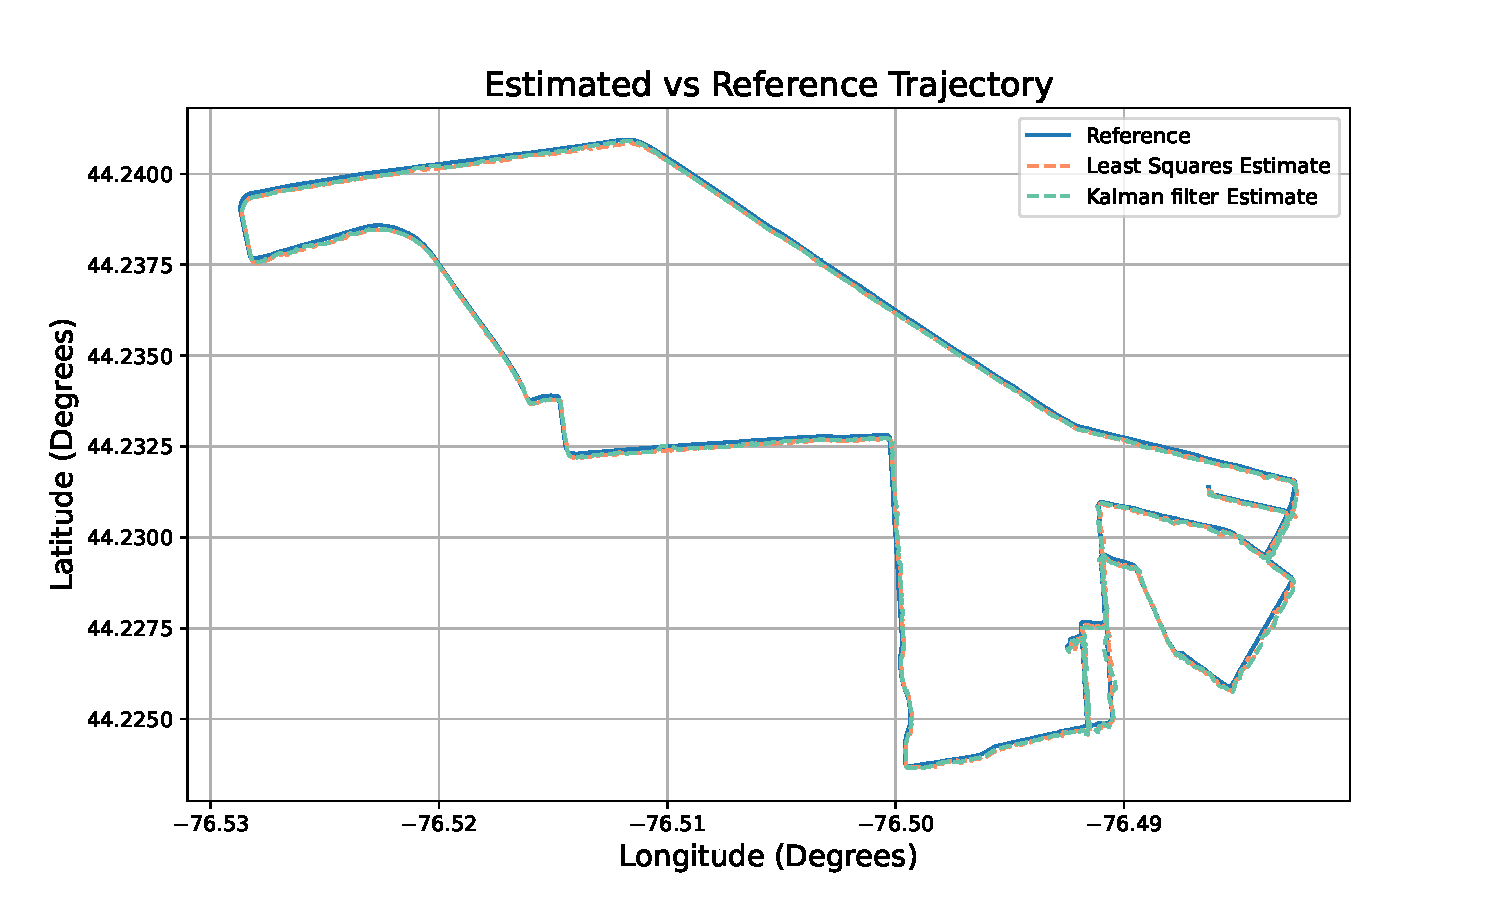
\includegraphics[width=0.5\textwidth]{plots/trajectory.pdf}}
\caption{Estimated Trajectory.}
\label{fig:traj}
\end{figure}

\begin{figure}[htbp]
\centerline{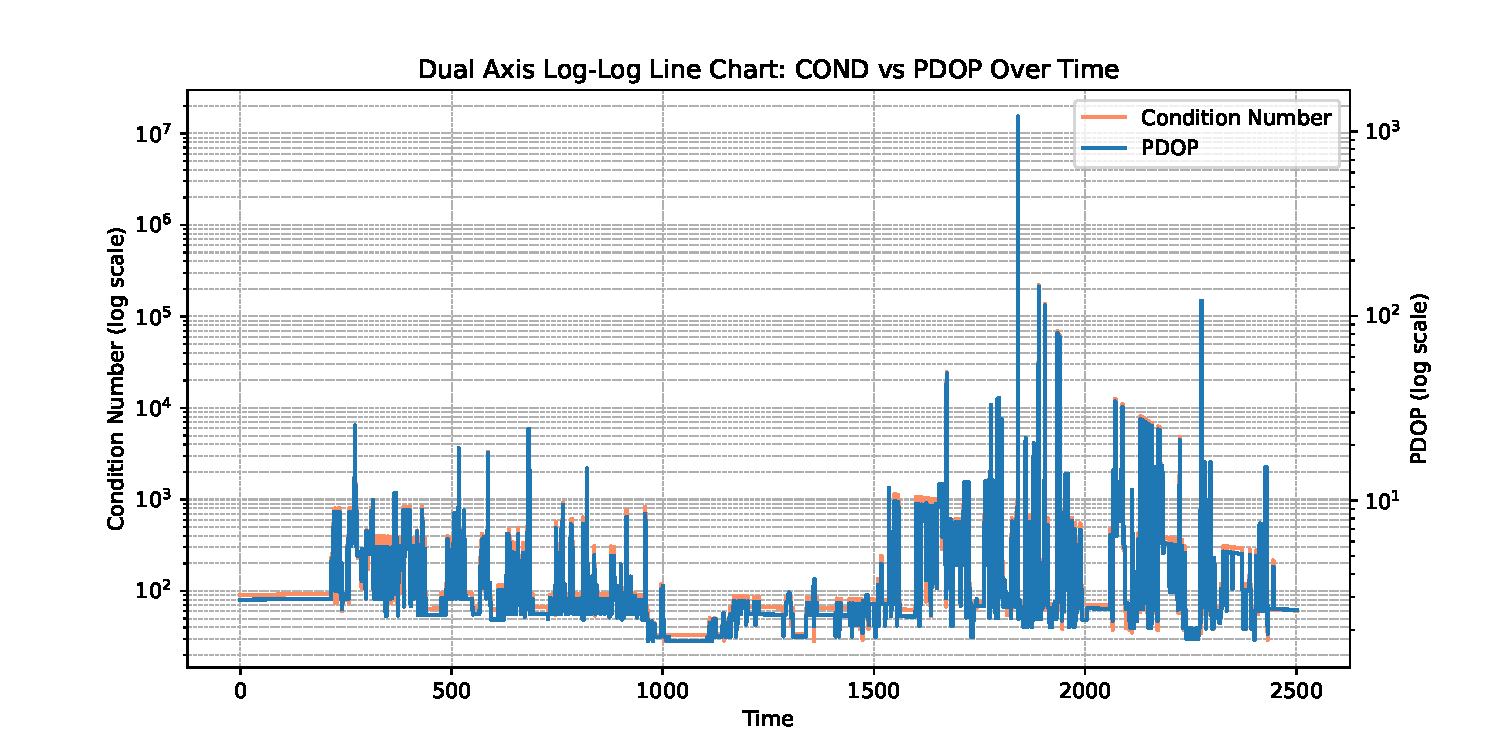
\includegraphics[width=0.5\textwidth]{plots/COND_DOP.pdf}}
\caption{Plots of DOP and its relation with Conditional Number of Jacobian.}
\label{fig:DOP COND}
\end{figure}

\begin{figure*}[htbp]
    \centering
    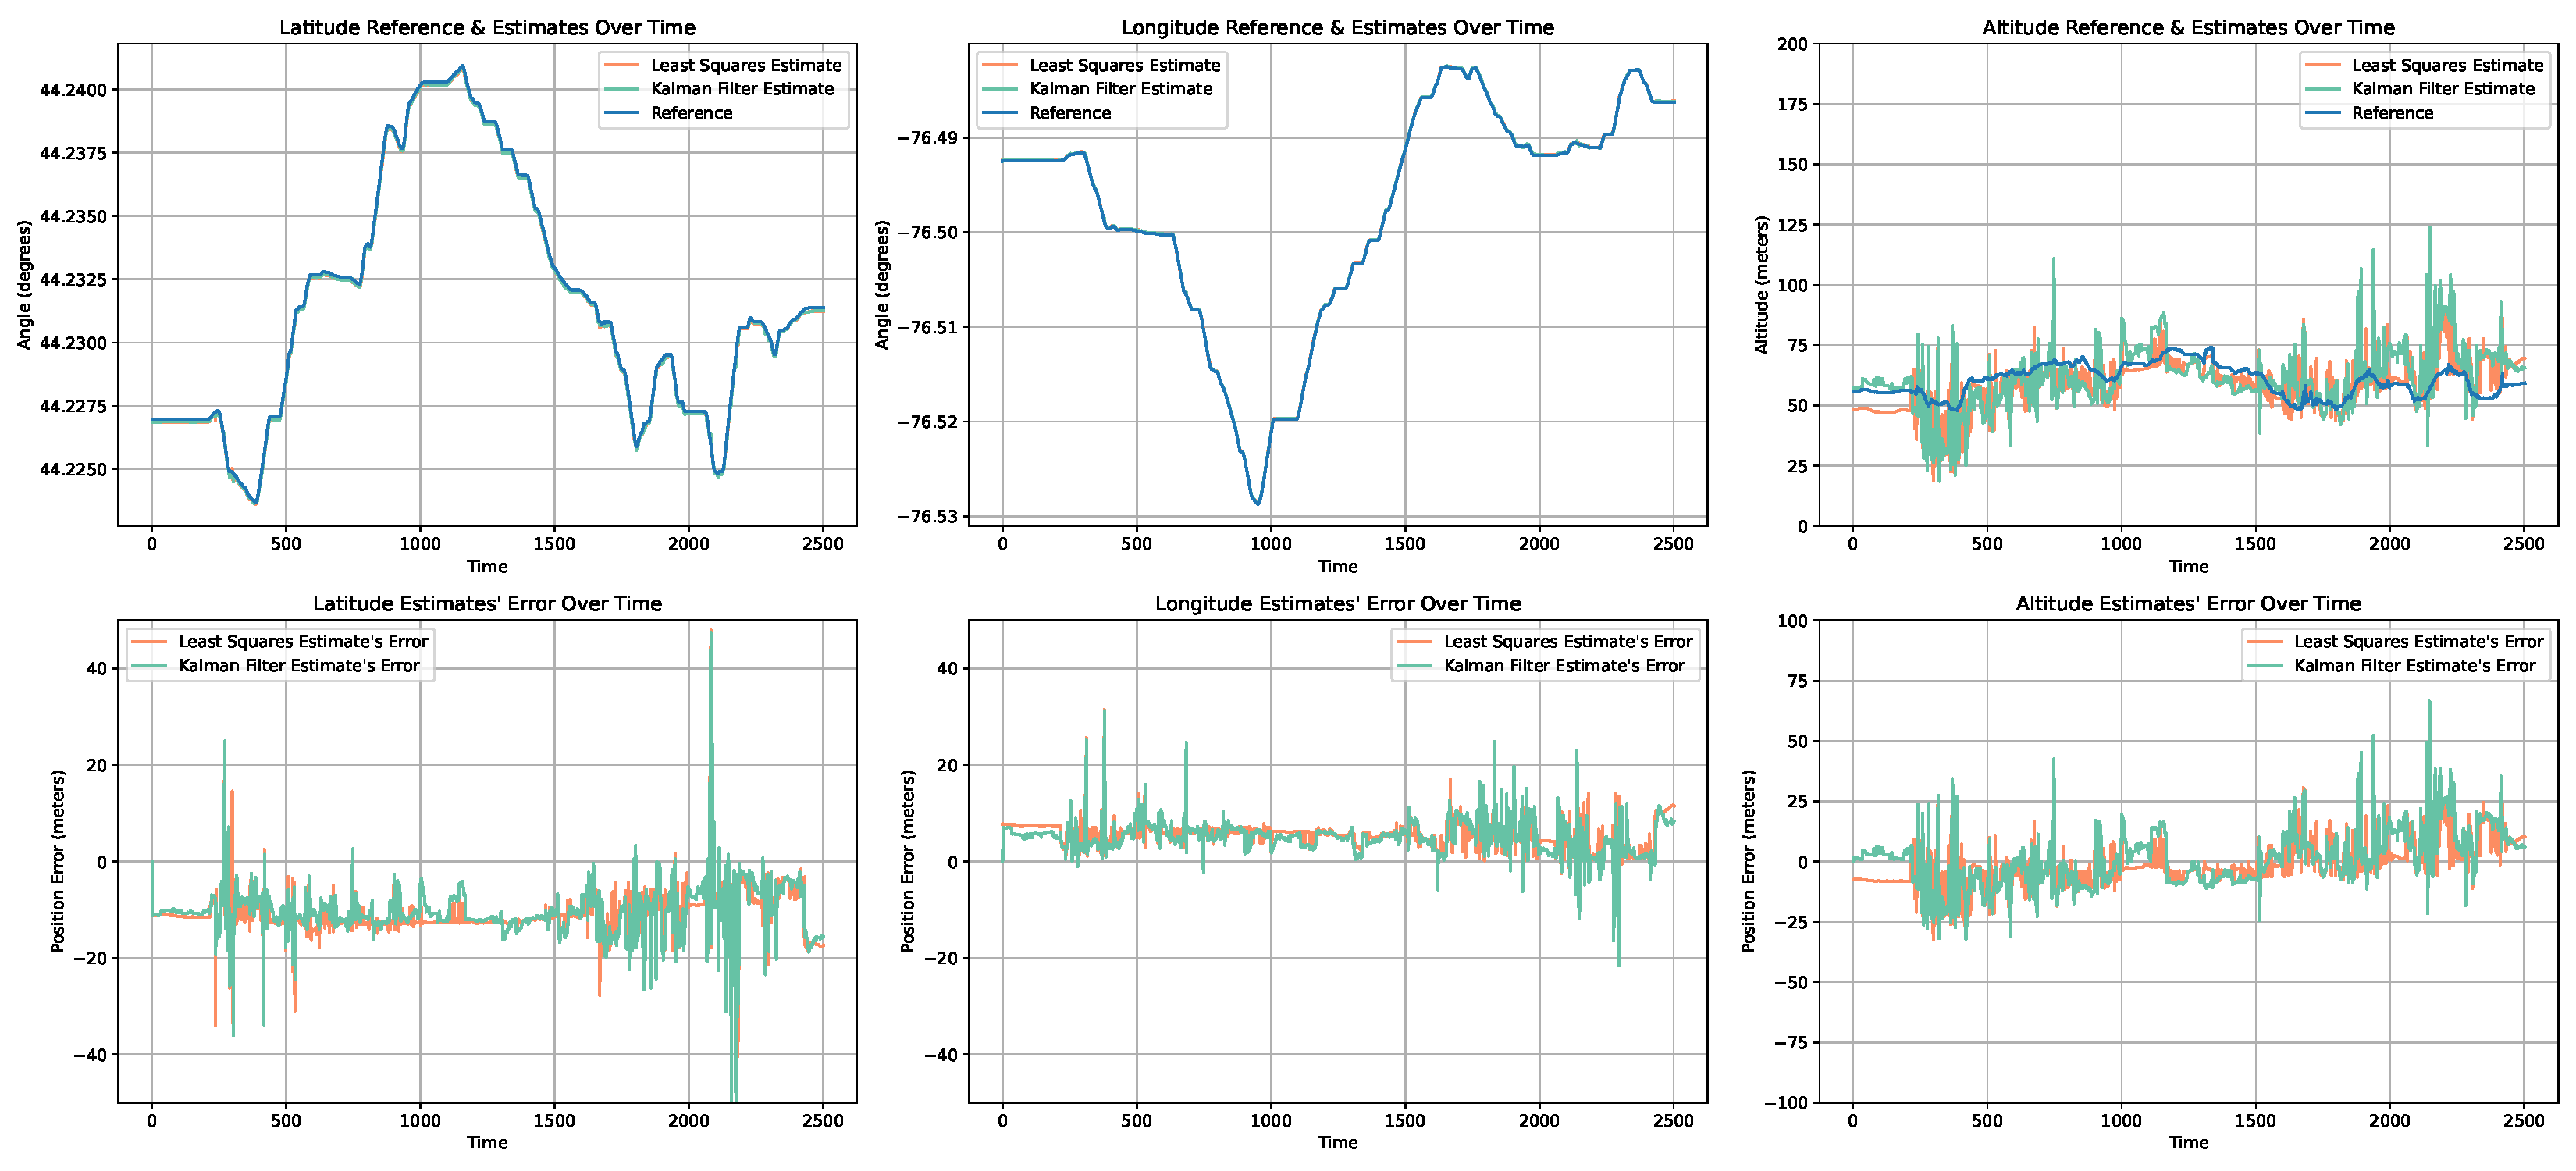
\includegraphics[width=1\textwidth]{plots/pos_err.pdf}
    \caption{Plots of Positional Components Estimates and their Errors by NLS and KF}
    \label{fig:Pos Err}
\end{figure*}

\begin{figure*}[htbp]
    \centering
    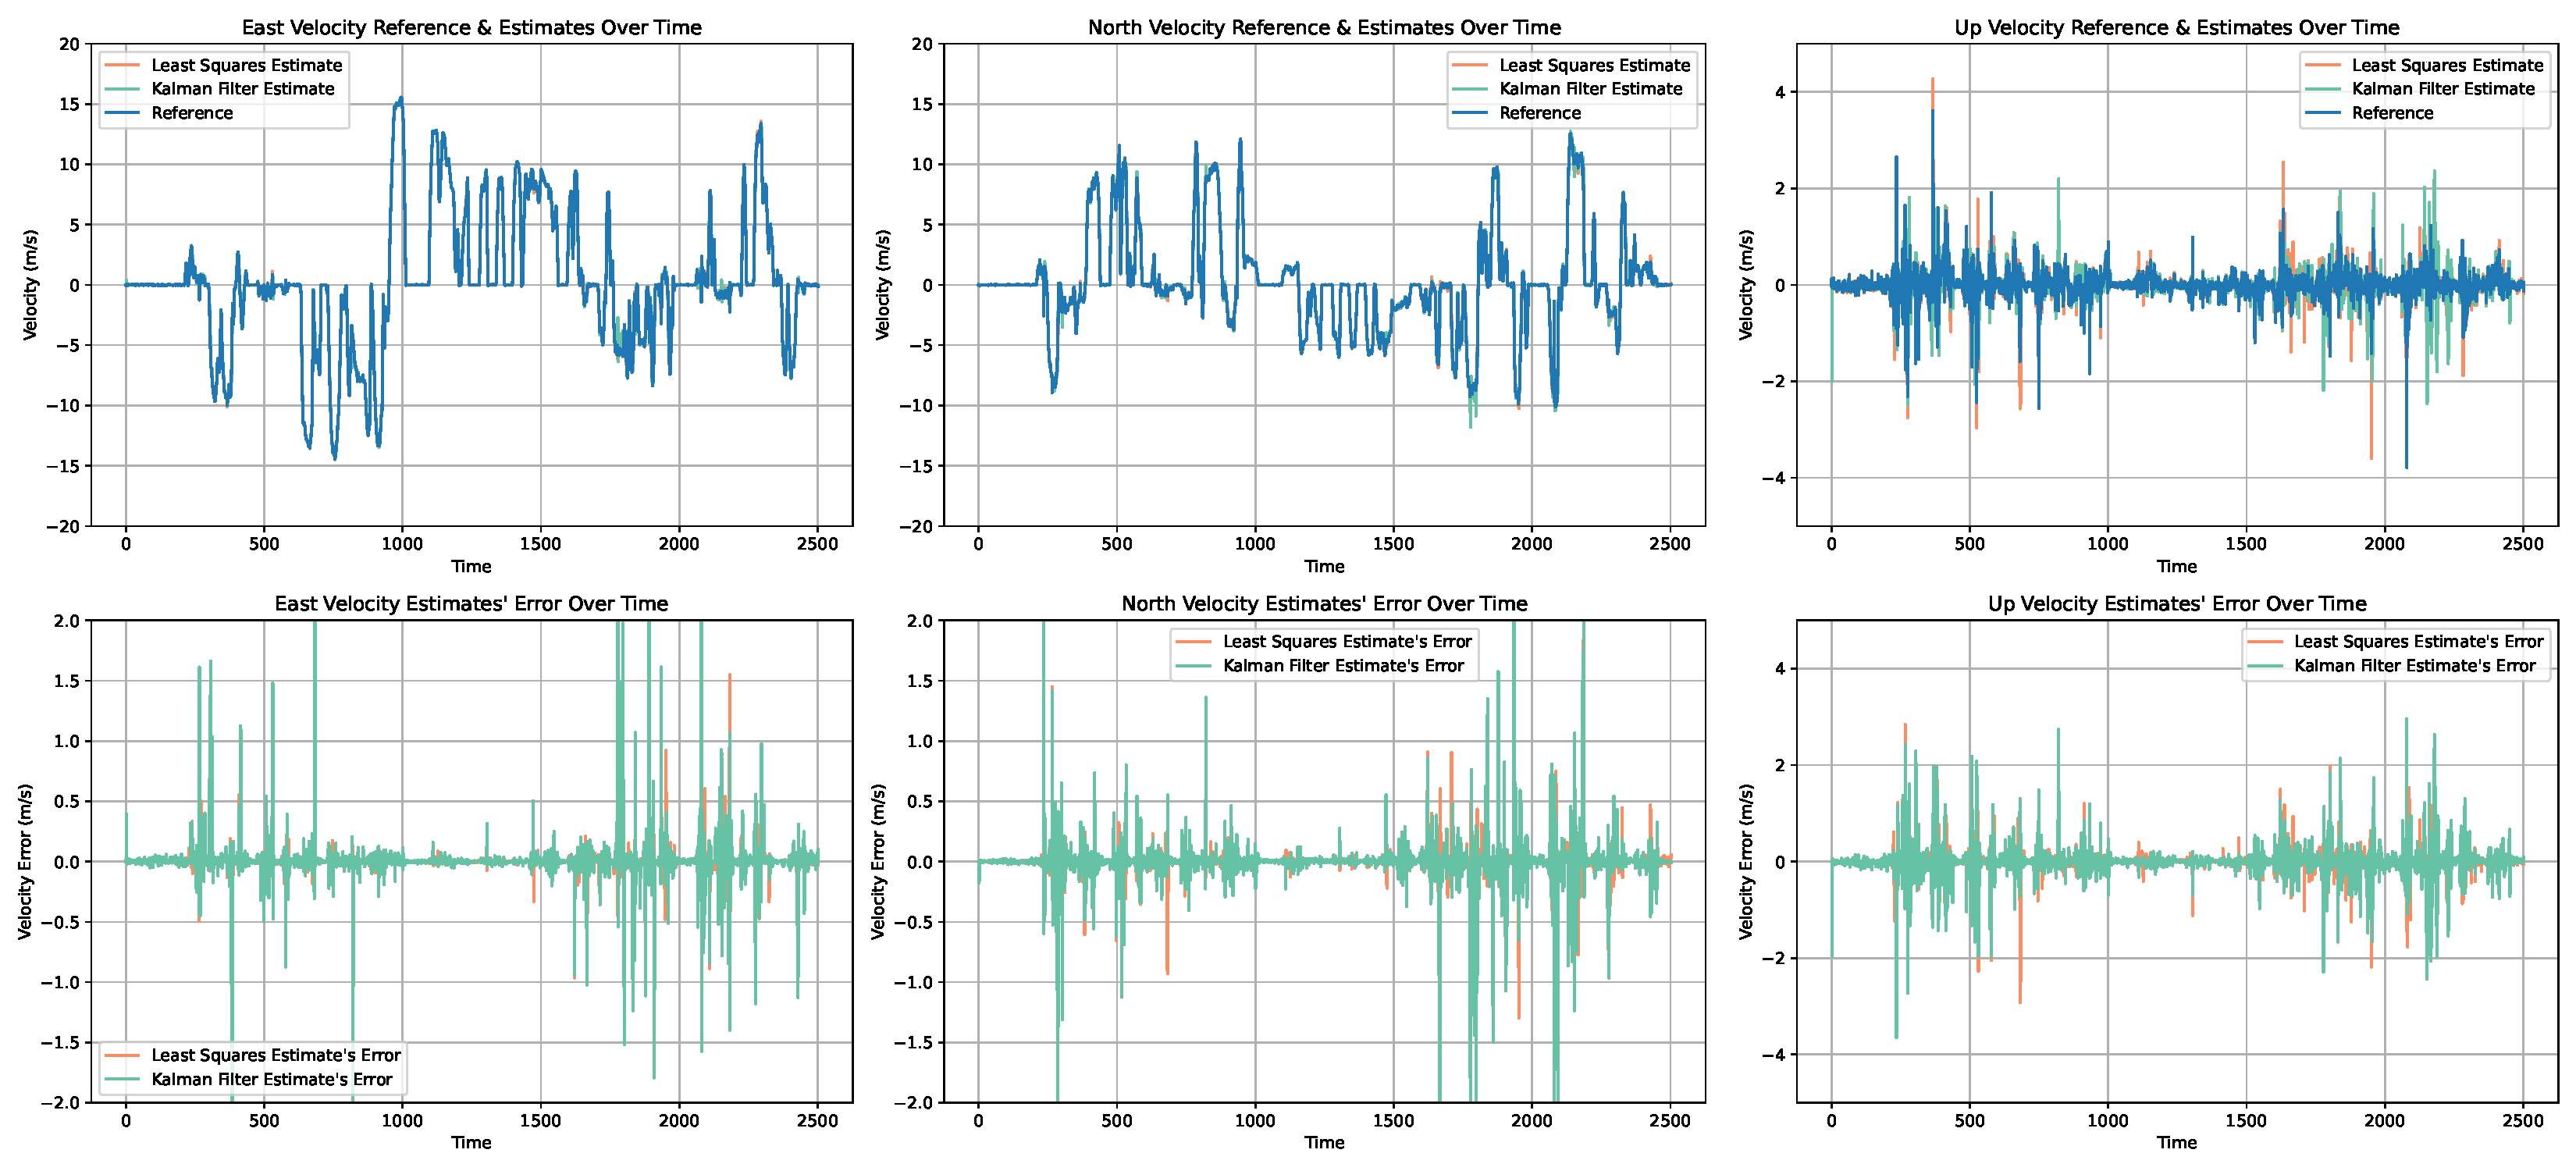
\includegraphics[width=1\textwidth]{plots/vel_err.pdf}
    \caption{Plots of Velocity Components Estimates and their Errors by NLS and KF}
    \label{fig:Vel Err}
\end{figure*}

\begin{figure*}[htbp]
    \centering
    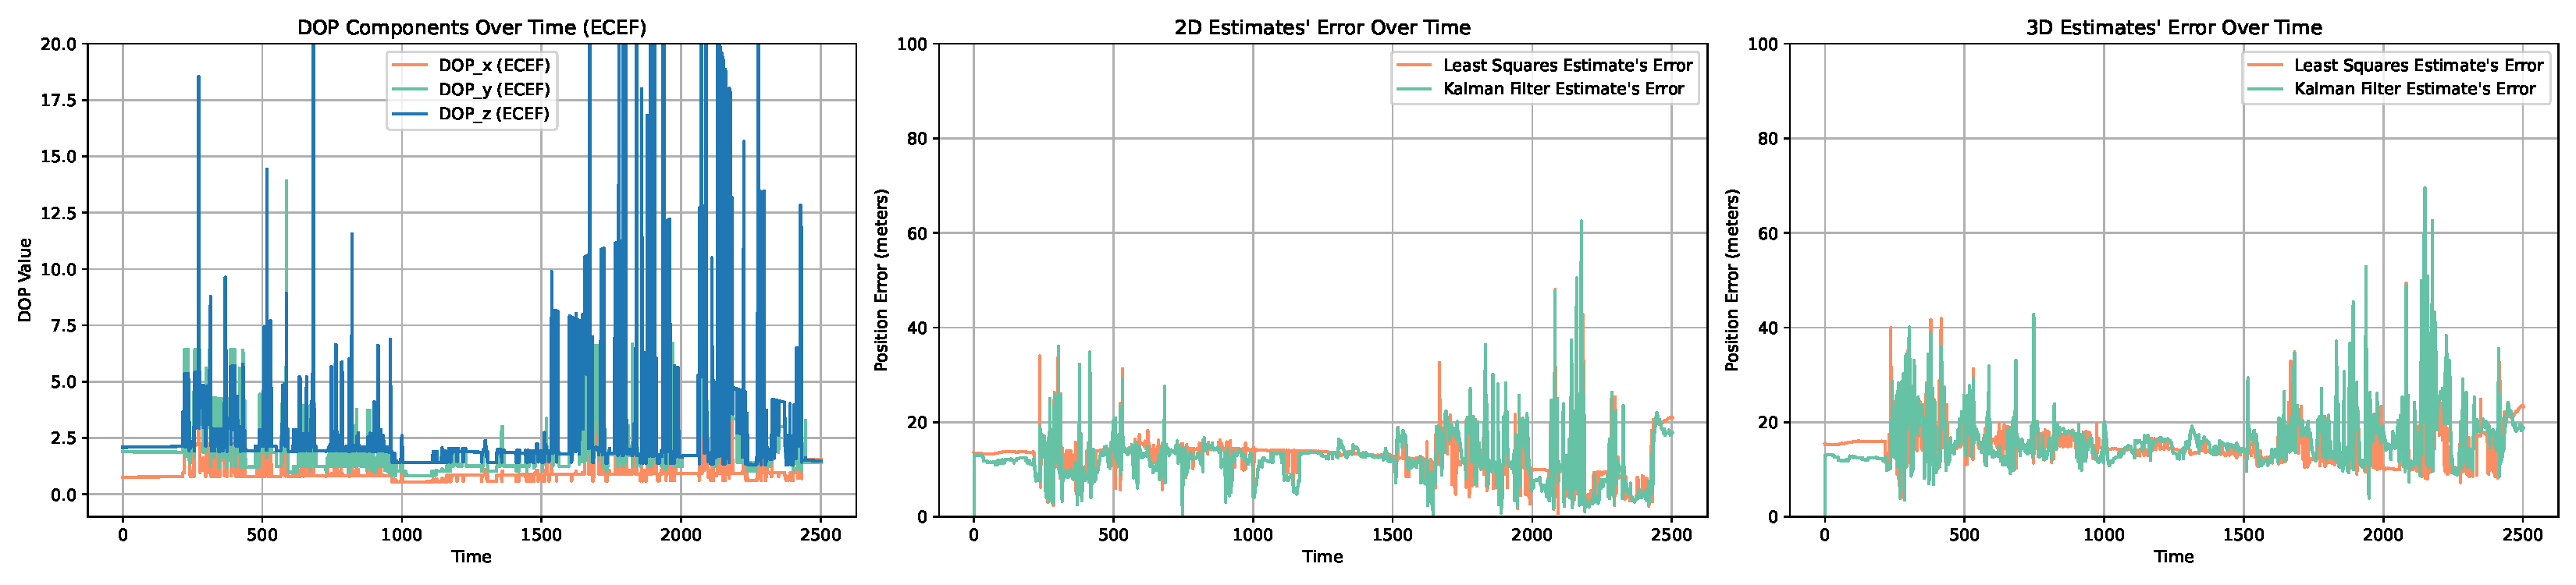
\includegraphics[width=1\textwidth]{plots/DOP2D3D.pdf}
    \caption{Plots of DOP and its relation with 2D and 3D Positional Error}
    \label{fig:DOP2D3D}
\end{figure*}

\begin{figure*}[htbp]
    \centering
    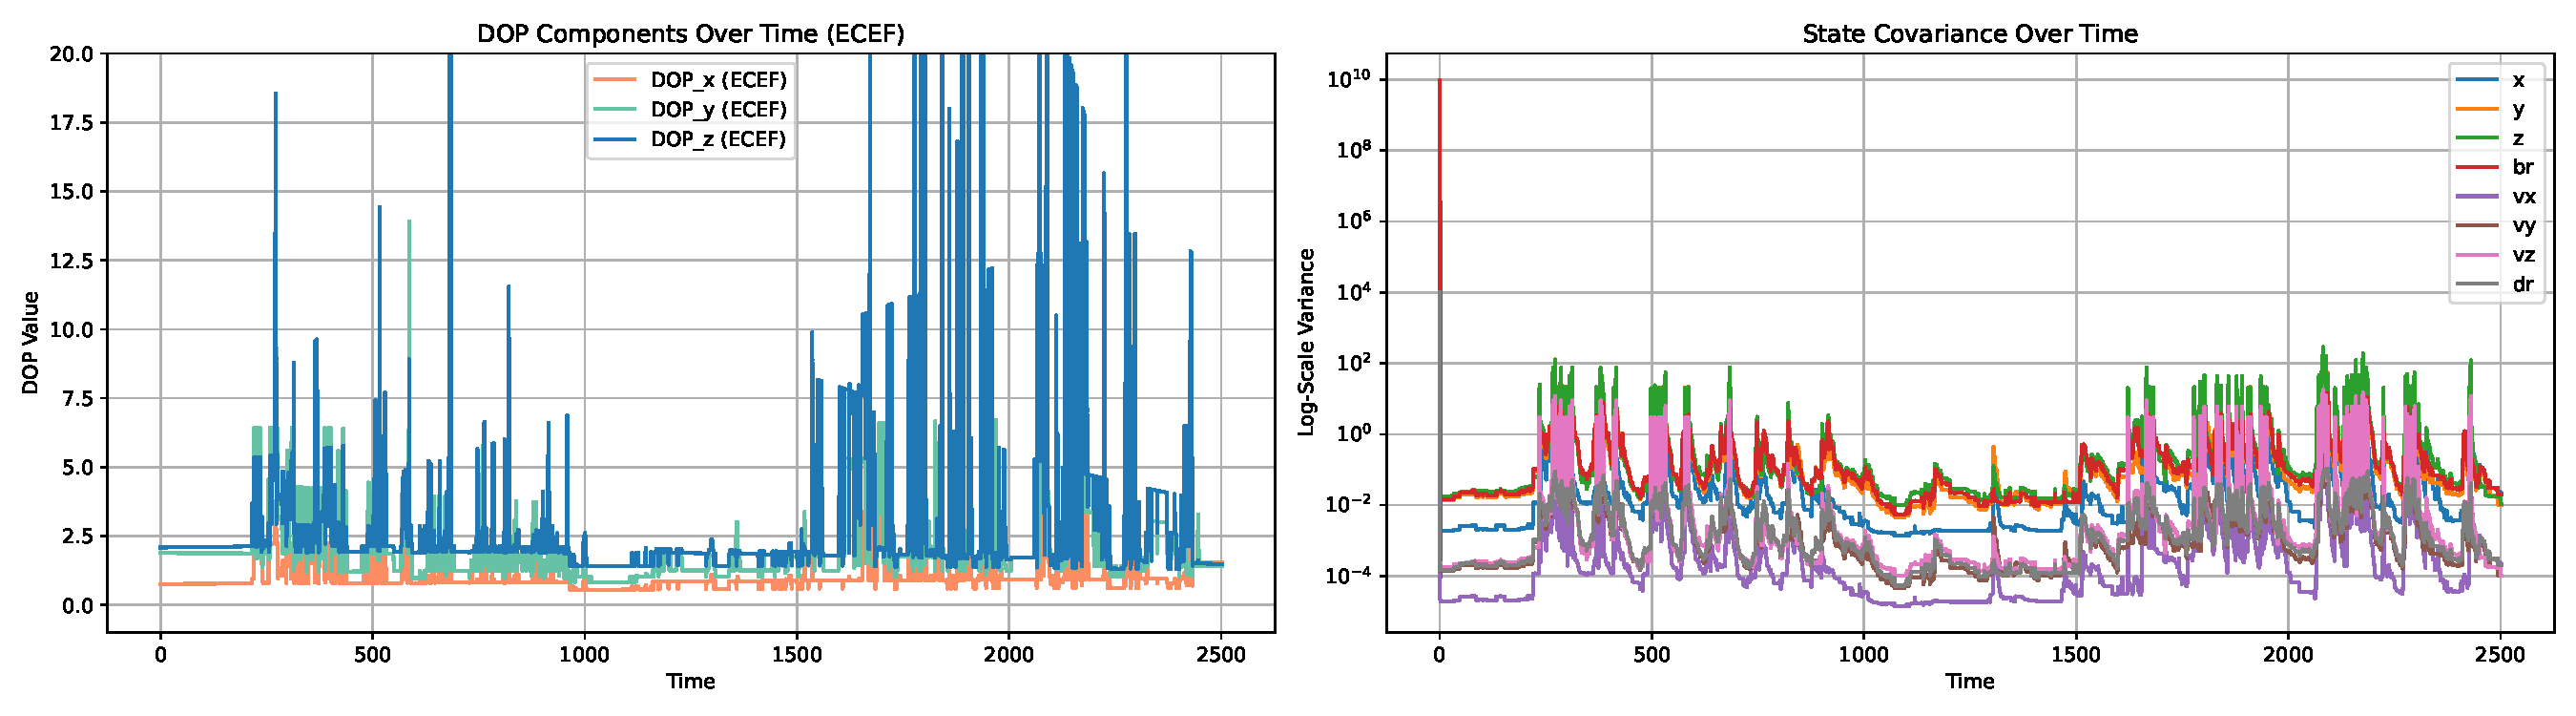
\includegraphics[width=1\textwidth]{plots/DOP_state_cov.pdf}
    \caption{Plots of DOP and its relation with Error State Covariance}
    \label{fig:DOP COV}
\end{figure*}

\begin{table*}[h!]
\centering
\begin{tabular}{|c|c|c|c|c|c|c|c|c|c|c|c|c|c|c|c|}
\hline
\textbf{Method} & \multicolumn{3}{c|}{\textbf{North}} & \multicolumn{3}{c|}{\textbf{East}} & \multicolumn{3}{c|}{\textbf{Altitude}} & \multicolumn{3}{c|}{\textbf{2D}} & \multicolumn{3}{c|}{\textbf{3D}} \\
\cline{2-16}
 & \textbf{Std} & \textbf{RMS} & \textbf{Max} & \textbf{Std} & \textbf{RMS} & \textbf{Max} & \textbf{Std} & \textbf{RMS} & \textbf{Max} & \textbf{Std} & \textbf{RMS} & \textbf{Max} & \textbf{Std} & \textbf{RMS} & \textbf{Max} \\
\hline
KF & 4.8 & \textbf{11.3} & \textbf{47.7} & 3.4 & 6.2 & 36.8 & 12.4 & 12.4 & 85.6 & 4.8 & \textbf{12.8} & 56.2 & 6.5 & 17.9 & 87.1 \\
\hline
DOP-Gated KF & 5.1 & 11.5 & 61.8 & 3.3 & \textbf{6.1} & \textbf{31.3} & 11.6 & 11.7 & 66.4 & 5.0 & 13.0 & 62.5 & 5.9 & 17.5 & 69.6 \\
\hline
GN-NE & 8.5 & 14.1 & 305.5 & 12.9 & 13.9 & 589.4 & 51.3 & 51.4 & 2428.0 & 14.3 & 19.8 & 663.9 & 51.8 & 55.1 & 2517.2 \\
\hline
WGN-NE & 8.3 & 13.4 & 305.5 & 12.8 & 13.8 & 589.4 & 51.2 & 51.2 & 2428.0 & 14.2 & 19.2 & 663.9 & 51.8 & 54.7 & 2517.2 \\
\hline
DOP-Gated WGN-NE & 4.8 & 12.0 & 60.1 & 2.8 & 6.3 & 31.5 & 8.9 & 9.0 & 32.6 & 4.6 & 13.5 & 61.0 & 4.5 & 16.2 & 61.0 \\
\hline
GN-QR & 8.5 & 14.1 & 305.5 & 12.9 & 13.9 & 589.4 & 51.3 & 51.4 & 2428.0 & 14.3 & 19.8 & 663.9 & 51.8 & 55.1 & 2517.2 \\
\hline
WGN-QR & 8.3 & 13.4 & 305.5 & 12.8 & 13.8 & 589.4 & 51.2 & 51.2 & 2428.0 & 14.2 & 19.2 & 663.9 & 51.8 & 54.7 & 2517.2 \\
\hline
GN-SVD & 4.7 & 12.5 & 48.0 & 3.0 & 6.5 & 31.5 & 9.8 & 9.8 & 52.5 & 4.5 & 14.0 & 48.1 & 4.2 & 17.1 & 52.6 \\
\hline
WGN-SVD & \textbf{4.3} & 11.7 & 48.0 & \textbf{2.7} & 6.2 & 31.5 & \textbf{8.9} & \textbf{9.0} & \textbf{32.6} & \textbf{4.2} & 13.2 & \textbf{48.1} & \textbf{4.2} & \textbf{16.0} & \textbf{49.4} \\
\hline
\end{tabular}
\caption{Error statistics for different methods (Std, RMS, and Max for North, East, Altitude, 2D, and 3D).}
\label{tab:error_stats}
\end{table*}

\begin{table*}[h!]
\centering
\begin{tabular}{|c|c|c|c|c|c|c|c|c|c|}
\hline
\textbf{Method} & \multicolumn{3}{c|}{\textbf{East Velocity}} & \multicolumn{3}{c|}{\textbf{North Velocity}} & \multicolumn{3}{c|}{\textbf{Up Velocity}} \\
\cline{2-10}
 & \textbf{Std} & \textbf{RMS} & \textbf{Max} & \textbf{Std} & \textbf{RMS} & \textbf{Max} & \textbf{Std} & \textbf{RMS} & \textbf{Max} \\
\hline
KF & 0.2 & 0.2 & 5.3 & 0.3 & 0.3 & 7.6 & 0.4 & 0.4 & 4.1 \\
\hline
DOP-Gated KF & 0.2 & 0.2 & 3.0 & 0.3 & 0.3 & \textbf{7.6} & 0.4 & 0.4 & 3.6 \\
\hline
GN-NE & 2.5 & 2.5 & 124.5 & 1.3 & 1.3 & 65.6 & 10.2 & 10.2 & 508.4 \\
\hline
WGN-NE & 2.5 & 2.5 & 124.5 & 1.3 & 1.3 & 65.6 & 10.2 & 10.2 & 508.4 \\
\hline
DOP-Gated WGN-NE & 0.2 & 0.2 & 2.8 & 0.3 & 0.3 & 7.7 & 0.3 & 0.3 & 3.6 \\
\hline
GN-QR & 2.5 & 2.5 & 124.5 & 1.3 & 1.3 & 65.6 & 10.2 & 10.2 & 508.4 \\
\hline
WGN-QR & 2.5 & 2.5 & 124.5 & 1.3 & 1.3 & 65.6 & 10.2 & 10.2 & 508.4 \\
\hline
GN-SVD & 0.2 & 0.2 & 2.4 & 0.3 & 0.3 & 7.7 & 0.3 & 0.3 & 3.6 \\
\hline
WGN-SVD & \textbf{0.2} & \textbf{0.2} & \textbf{2.4} & \textbf{0.2} & \textbf{0.2} & 7.7 & \textbf{0.3} & \textbf{0.3} & \textbf{3.6} \\
\hline
\end{tabular}
\caption{Error statistics for different methods (Std, RMS, and Max for East, North, and Up).}
\label{tab:velocity_error_stats}
\end{table*}


\section{Discussion}

\subsection{Addressing The Effect of System Geometry \& System Conditioning}

The sources of error in our problem can be broadly categorized into two main factors: \textbf{unreliable measurements} (such as multipath effects, low-elevation satellites, and unmodeled atmospheric effects) and \textbf{system conditioning} issues related to the geometry of the satellites and receivers, typically quantified using Dilution of Precision (DOP).

From numerical linear algebra \cite{trefethen1997}, it is well known that a \textbf{high condition number for the Jacobian matrix} severely affects the quality of nonlinear estimates. In our problem, \textbf{the Jacobian matrix corresponds to the geometry matrix, which fully captures the relative positioning between the receiver and the visible satellites}. Figure \ref{fig:DOP COND} demonstrates a strong correlation between the condition number and PDOP (Position Dilution of Precision). Specifically, epochs with poor satellite geometry—such as satellites clustered in one direction or exhibiting collinearity—tend to have a high condition number, leading to degraded estimate quality.

From Figure \ref{fig:DOP2D3D}, we can clearly observe that 2D and 3D positional errors correlate directly with PDOP. Additionally, from Figure \ref{fig:DOP COV} we can see that for the epochs with high PDOP and condition numbers, the error-state covariance matrix increases the variances of the estimates, until it stabilizes again when measurements become well-conditioned.

A comparison between the basic Kalman Filter (KF) implementation and Nonlinear Least Squares with normal equation-based inversion (GN-NE) reveals significant spikes in the maximum error statistics for GN-NE compared to the Kalman Filter. These error spikes correspond to epochs with poor satellite geometry. The Kalman Filter, being recursive in nature, has inherent smoothing properties (as described in Bayesian filtering), which help mitigate the effects of ill-conditioned epochs more effectively than GN-NE. This explains the large discrepancy between the basic Kalman Filter and GN-NE implementations.

From the tabulated positional errors, we can also observe that 3D positional error is primarily dominated by altitude errors. This aligns with the plot, where $DOP_z$ exhibits the highest spikes, indicating that uncertainty in the z-dimension significantly impacts altitude estimates. Additionally, the tabulated results reveal a \textbf{directional bias in horizontal positioning}—North estimates are worse than East estimates. This is because the North component is linked to latitude, which has a strong dependence on the z-dimension of the ECEF (Earth-Centered, Earth-Fixed) frame, whereas the East component is linked to longitude, which has no contribution from the z-dimension in ECEF.

Given these observations, we see a substantial performance boost when DOP-Gating is applied to GN-NE (DOP-Gated GN-NE). By filtering out epochs with excessively high PDOP, DOP-Gating prevents the inversion of ill-conditioned systems, thereby improving overall robustness. However, its effect on Kalman filtering is less pronounced, since the Kalman Filter already incorporates smoothing mechanisms to handle ill-conditioned estimates.

\subsection{Limitations of DOP-Gating:}
A key drawback of DOP-Gating is that it completely discards data from epochs with PDOP exceeding a threshold. This means that valuable information is lost, and state estimates must be approximated from previous epochs. This can be particularly problematic for fast-moving vehicles, where outdated estimates may lead to inaccuracies.

\subsection{Addressing the Normal Equation Inversion Problem:}
The primary limitation of GN-NE lies in its reliance on normal equation-based inversion. The term $\tilde{\mathbf{G}^T} \tilde{\mathbf{G}}$squares already small singular values, further worsening the conditioning of the system in epochs with high PDOP. Consequently, methods that avoid this squaring effect, such as QR decomposition and Singular Value Decomposition (SVD), offer more stable solutions for ill-conditioned systems.

\subsubsection{Comparing GN-SVD and GN-QR}
From the tabulated results, GN-SVD significantly outperforms GN-QR. This is because QR decomposition does not have the regularization effect of truncating near-zero singular values, which are critical for system conditioning. While QR is computationally faster, SVD remains the more robust and reliable method for solving severely ill-conditioned linear systems.

\subsection{The Impact of Weighting:}
Additionally, weighted SVD (WGN-SVD) provides further improvements over GN-SVD. This result aligns with theoretical expectations since WGN-SVD does not assume homoscedasticity, unlike ordinary least squares (OLS). Since low-elevation satellites are more susceptible to unmodeled atmospheric degradation, their corresponding pseudorange and Doppler measurements have higher variances. Weighted SVD appropriately accounts for these variations, improving accuracy.

In summary, WGN-SVD significantly closes the performance gap and surpasses the DOP-Gated Kalman Filter, making it the preferred method.

\section{Future Work}

Future work could explore alternative solvers for the Nonlinear Least Squares (NLS) problem, specifically Levenberg-Marquardt (LM) for improved handling of ill-conditioned systems and Newton’s Method, a full second-order approach that does not approximate the Hessian, offering greater robustness.

Additionally, for the Kalman Filter, the Square Root Kalman Filter (SRKF) variant could be beneficial, as it enhances numerical stability and better manages ill-conditioned systems.

\section{Conclusion}

GNSS point positioning is indispensable for establishing a robust and reliable navigation solution, serving as the backbone for various applications in transportation, geodesy, and autonomous systems. Given its significance, ensuring accurate and stable positioning remains a fundamental challenge.

At its core, GNSS point positioning is a classical state estimation problem, typically solved using Kalman Filtering (KF) or Nonlinear Least Squares (NLS). Both methods aim to estimate receiver states using satellite observations, but their performance is highly dependent on system conditioning, which is largely dictated by relative satellite-receiver geometry.

The Dilution of Precision (DOP) metric quantifies the effect of satellite geometry on system conditioning, directly influencing the quality of the estimated receiver position. Poor satellite geometry, characterized by high DOP values, can severely degrade positioning accuracy by amplifying numerical instability. While Kalman Filtering, due to its recursive smoothing properties, partially mitigates these effects, the same DOP spikes pose a significant challenge to NLS solutions, leading to large errors.

To address this, a DOP-Gated Epoch Rejection heuristic was employed, successfully curbing the influence of high DOP values by discarding poorly conditioned epochs. However, this approach comes at the cost of losing valuable measurement data, which can negatively impact accuracy, particularly in dynamic environments where rapid state updates are critical.

To further improve robustness, alternative inversion techniques were explored. In particular, Singular Value Decomposition (SVD)-based inversion provided a substantial performance boost, demonstrating superior handling of ill-conditioned systems compared to normal equation-based and QR-based inversions. By avoiding the squaring of small singular values, SVD ensures numerical stability and better conditioning of the system.

Additionally, measurement weighting introduced further improvements over standard least squares. Unlike Ordinary Least Squares (OLS), which assumes homoscedasticity (equal variance in all measurements), the Weighted GNSS approach accounts for satellite-specific uncertainties, such as increased measurement noise from low-elevation satellites affected by atmospheric disturbances.

\begin{thebibliography}{00}

\bibitem{noureldin2013} A. Noureldin, T. B. Karamat, and J. Georgy, \textit{Fundamentals of Inertial Navigation, Satellite-Based Positioning and Their Integration}. Berlin, Germany: Springer-Verlag, 2013.

\bibitem{trefethen1997} L. N. Trefethen and D. Bau III, \textit{Numerical Linear Algebra}. Philadelphia, PA, USA: SIAM, 1997.


\end{thebibliography}

\end{document}
